\documentclass[a4paper,12pt,oneside]{report}%pridat twoside, do [] pre obojstrannu tlac
    \pagestyle{headings}
    \usepackage[top=2.5cm, bottom=2.5cm, left=3.5cm, right=2cm]{geometry} %odporucane okraje
	\linespread{1.50}

\usepackage[T1]{fontenc} %pekne makcene
\usepackage{amsmath}
\usepackage{mathtools}
\usepackage{amssymb}
\usepackage{graphicx}
\usepackage{graphics}
\usepackage{algorithmic}
\usepackage{algorithm}
\usepackage{listings}
%\usepackage{cite}

\graphicspath{ {pictures/} }
\renewcommand{\thesection}{\arabic{section}}

\author{Mat\'u\v{s} Behun}
\title{Cayley graphs of given diameter or girth on linear groups}

\usepackage{hyperref}
    \hypersetup{colorlinks,citecolor=red,filecolor=black,linkcolor=blue,urlcolor=blue,pdftex}

\begin{document}
\setlength{\belowdisplayskip}{7pt} \setlength{\belowdisplayshortskip}{5pt}
\setlength{\abovedisplayskip}{7pt} \setlength{\abovedisplayshortskip}{5pt}

%====================================================================================================================================================
% FIRST PAGE
%====================================================================================================================================================

\thispagestyle{empty}
{
     \topmargin=0pt
     \centerline {\large \bf{Slovak University of Technology in Bratislava}}
     \vskip 0.2cm
     \centerline{\large \bf{Faculty of Civil Engineering}}
     \vskip 5cm
     \centerline{\Large \bf{Cayley graphs of given degree and diameter on linear groups}}
     \vskip 0.2cm
     \vskip 0.5cm
     \centerline{\large \bf{Bachelor Thesis}}
     \vskip 5cm          %\vskip 2cm             %zmena kvoli zobrazovaniu dnesneho datumu
     \normalsize
         \begin{tabular}[l]{p{0.27\textwidth}p{0.73\textwidth}}
			 \v{S}tud\'ijny program: & Matematicko-po\v{c}ita\v{c}ov\'e modelovanie \\
         	\v{S}ud\'ijny odbor: & Aplikovan\'a matematika \\
         	\v{S}koliace pracovisko: & Katedra matematiky a deskript\'ivnej geometrie \\
			 Ved\'uci z\'avere\v{c}nej pr\'ace: & Jana \v{S}iagiov\'a \\
         \end{tabular}
     \vskip 3cm
     \centerline{\large \bf{Bratislava 2018}}
     \vskip 0.2cm
	 \centerline{\large \bf{Mat\'u\v{s} Behun}}
}

 \newpage

%====================================================================================================================================================
% END OF FIRST PAGE
%====================================================================================================================================================

\section{Abstract}

This bachelor thesis discuss two problems concerning construction of graphs with given restriction, namely {\em degree/diameter} and {\em degree/girth} problem. In our work we describe both problems, the associated theoretical bounds and some research results with focus on Cayley graphs on 2-dimensional special linear groups over finite fields. We present algorithm for generating such Cayley graphs of diameter 2, looking for smallest possible degree. We used randomized search over generating sets of predetermined sizes in small special linear groups of dimension 2 over finite fields.

\newpage

\section{Introduction}

In its simplest form, networks can be modeled by graphs in a natural way in which network nodes are represented by vertices of the graph and links between nodes are represented by undirected edges of the graph. Restrictions on the network, such as limits on the number of links attached to a node, or limits on the number of links needed to connect any two nodes, or the length of a shortest circuit, then transform to restrictions on the graph model (for the indicated cases these would be restrictions on vertex degrees, on the diameter, and on the girth of the graph).
\medskip

In graph theory this leads to two important problems: the {\em degree/diameter problem} to construct the largest possible graphs of a given maximum degree and a given diameter, and the {\em degree/girth problem} to construct the smallest possible regular graphs of a given degree and a given girth; in both cases the adjectives `large' and `small' refer to the order (i.e., the number of vertices) of a graph. The survey papers \cite{Mil-Sir} and \cite{Exo-Jaj}, respectively, contain a large amount of information on both problems. In this work we address both problems restricted to Cayley graphs of certain two-dimensional linear groups, giving details in what follows.


\newpage

%====================================================================================================================================================
% INTRODUCTION TO DEGREE DIAMETER PROBLEM ON UNDIRECTED GRAPHS strana 8, 9
%====================================================================================================================================================

\section{The degree/diameter problem}
\subsection{The Moore bound}

There is theoretical upper bound named after E. F. Moore for the largest order of a graph with given diameter $k\ge 1$ and maximum degree $d\ge 2$, which one can derive by building a spanning tree of such a graph. A fixed vertex $v$ of such a graph has at most $d$ neighbours at distance $1$. Each of these neighbours has at most $d-1$ vertices at distance $1$ from themselves, giving at most $d(d-1)$ vertices at distance $2$ from $v$. Iterating this process ne obtains at most $d(d-1)^{i-1}$ vertices at distance $i$ from $v$. By the diameter requirement, we have at most $d(d-1)^{k-1}$ vertices at distance $k$ from $v$. Summing up, the largest order $n_{d,k}$ of a graph of maximum degree $d\ge 2$ and diameter $k\ge 1$ is at most $M_{d,k}$, the Moore bound for the pair $(d,k)$, where

\begin{equation}\label{eq:Moore}
	\begin{split}
		n_{d,k} \leq M_{d,k}	& = 1 + d + d(d - 1) + \dots + d(d - 1)^{k-1}  \\
				 				& = 1 + d(1 + (d - 1) + \dots + (d - 1)^{k-1}) \\
				 				& =	\begin{cases}
										1+d\frac{(d-1)^{k}-1}{d-2}, & \text{if}\ d > 2 \\
										2k+1, & \text{if}\ d=2
									\end{cases}
	\end{split}
\end{equation}

%% About upper boundary
\subsection{Moore graphs}
It is well known that equality in (\ref{eq:Moore}) holds only if $d=2$ (for any $k\ge 1$), or $k=1$ (for any $d\ge 2$), or for $k=2$ and $d\in \{3,7\}$, and possibly for the pair $(d,k)=(57,2)$ but for no other $d\ge 2$ and $k\ge 1$. All the graphs for which $n_{d,k}=M_{d,k}$ are called {\em Moore graphs}; they are necessarily regular and in the order of the listed parameters they are cycles of length $2k+1$, complete graphs of order $d+1$, the Petersen graphs and the Hoffman-Singleton graph.
\medskip

Research into the degree/diameter problem and into Moore graphs in particular was initiated by Hoffman and Singleton in \cite{Hof-Sin} who proved that Moore graphs of diameter $k=2$ can exist only for $d\in \{2,3,7\}$ and possibly $57$, proving also their uniqueness except for the last case, and establishing also that the unique Moore graph of diameter $3$ is the cycle of length $7$. Their proofs exploit eigenvalues and eigenvectors of adjacency matrices (and the corresponding principal submatrices) of graphs.
\medskip

\begin{figure}[!ht]
	\centering
	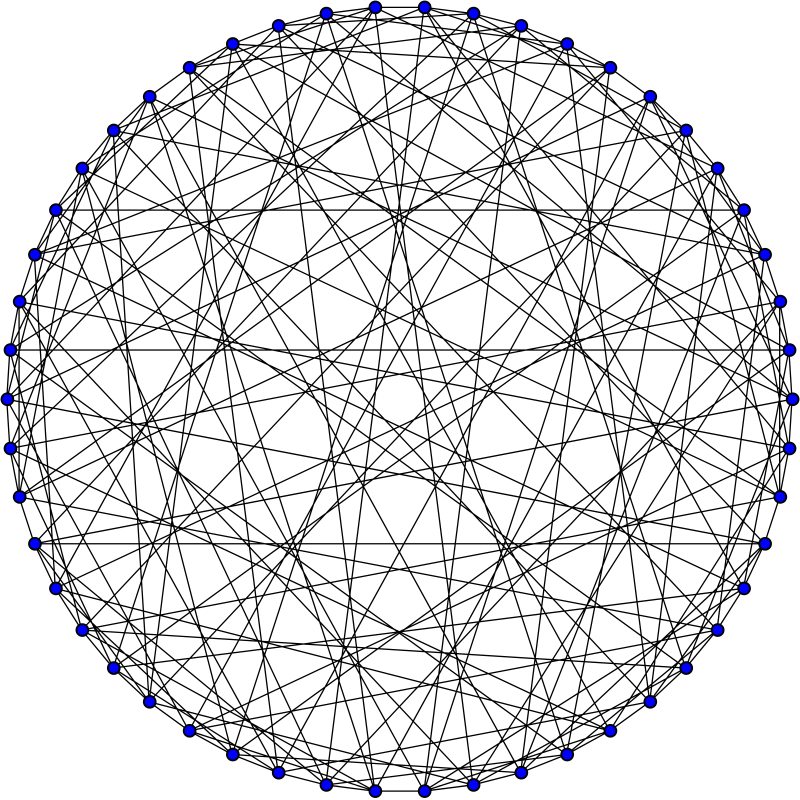
\includegraphics[scale=0.33]{Hoffman-Singleton_graph.png}
	\caption{Hoffman-singleton graph is Moore graph with $d=7$ and $k=2$ }
\end{figure}

%====================================================================================================================================================
% END OF INTRODUCTION TO DEGREE DIAMETER PROBLEM
%====================================================================================================================================================

%====================================================================================================================================================
% GRAPHS NON MOORE'S
%====================================================================================================================================================

\subsection{Graphs of order close to the Moore bound}
To facilitate the explanations, any graph of maximum degree $d$ and diameter $k$ will be called a $(d,k)$-{\em graph}. Because for $d\ge 3$ and $k\ge 2$ there are only a few $(d,k)$-graphs of order equal to the value $M_{d,k}$ of the Moore bound, researchers have tried to construct $(d,k)$-graphs of order as close to $M_{d,k}$ as possible. For a $(d,k)$-graph of order $M_{d,k}-\delta$ the quantity $\delta$ is knwn as the {\em defect}, and then we speak about a $(d,k,-\delta)$-graph; we note that this terminology is only used for `small' defects.
\medskip

There are a number of results concerning graphs with small defect. For example, Erd\"os, Fajtlowitcz and Hoffman proved \cite{Erd-Faj} that there is no graph of degree $d$ and diameter $2$ with $\delta = 1$ apart from the cycle of length $4$. In the case of $\delta = 2$ and $d = 2$ all the $(d,k,-2)$-graphs are the cycles of length $2k-1$. For $\delta-2$ and $d \geq 3$ only five graphs are known at present, namely, two $(3,2,-2)$-graphs of order $8$, one $(4,2,-2)$-graph of order $15$, one $(5,2,-2)$-graph of order $24$, and one $(3,3,-2)$-graph of order $20$; for details we refer to \cite{Mil-Sir}.

\subsection{Constructions of large graphs}
A different approach to finding $(d,k)$-graphs of order close to the Moore bound is by constructing appropriate `large' $(d,k)$-graphs. In most cases the constructions use combinatorics on words or algebraic structures such as groups and fields, so that the resulting graphs turn out to be rich in symmetries, or even vertex-transitive (and sometimes even Cayley).
\medskip

For a long time one of the asymptotically best families was the one of the \textit{undirected de Brujin graphs}, which are $(d,k)$ graphs for even $d$ and yield the lower bound
\begin{equation*}
	n_{d,k} \geq \left( \frac{d}{2} \right)^{k}.
\end{equation*}

This bound was improved by Baskoro and Miller \cite{Bas-Mil} to
\begin{equation}
	n_{d,k} \geq \left( \frac{d}{2} \right)^{k} +  \left( \frac{d}{2} \right)^{k-1}
\end{equation}	

In the special case of diameter $k=2$, modified Brown graphs can give for sufficiently large $d$ the bound
\begin{equation*}
	n_{d,2} \geq d^{2} - 2d^{1+\varepsilon}
\end{equation*}	
where the number $\varepsilon < 1$ depends on results about gaps between consecutive prime numbers; see \cite{Bev-Ers} for details about the current development.

\subsection{Graph lifting}
Graph lifting is a technique by which one may produce `large' graphs with certain required properties from suitable `small' graphs. The technique is well-known in topological and algebraic graph theory and for historical and mathematical details we refer to the monograph \cite{Gro-Tuc}. The technique can be described in the language of the so-called voltage assignments, which we briefly present next.
\medskip

Let $G$ be a graph. Although our graphs are undirected, we will preassign a direction to every edge. An edge with a preassigned direction is an {\em arc}. If $e$ is an arc of $G$, by the symbol $e^{-1}$ we denote the {\em reverse} of $e$, obtained simply by changing the preassigned direction on the edge. Let $D(G)$ be the set of all arcs of $G$; it follows that the size of $D(G)$ is twice the number of edges of $G$.
\medskip

Let $G$ be a graph as above and let $\Gamma$ be a finite group. The mapping
\begin{align*}
	\alpha: D(G) \rightarrow \Gamma
\end{align*}	
will be called a {\em voltage assignment} if $\alpha(e^{-1})$ = $(\alpha(e))^{-1}$, for any arc $e \in D(G)$.
\medskip

Out of the graph $G$ and the voltage assignment $\alpha$ as introduced above one can construct a `larger' graph, called the {\em lift} of $G$ (under the assignment $\alpha$) and denoted $G^{\alpha}$. The vertex set and the dart set of the new graph are defined as follows:
\begin{align*}
	V(G^{\alpha}) = V(G) \times \Gamma \\
	E(G^{\alpha}) = E(G) \times \Gamma
\end{align*}	
with the condition that if an arc $e$ emanates from a vertex $u$ and terminates in a vertex $v$ in the {\em base graph} $G$, then for every $g\in \Gamma$ there is a dart $(e,g)$ emanating from the vertex $(u,g)$ and terminating in the vertex $(v,g\alpha(e)$. It follows that right multiplication by $\alpha(e)$ permutes the terminal vertices of arcs $(e,g)$ emanating from the vertices $(u,g)$. At the same time this right multiplication induces a group of automorphisms of the lift acting freely on vertices and isomorphic to the {\em voltage group} $\Gamma$. Note that $G^{\alpha}$ can be considered to be an undirected graph, because the arcs $(e,g)$ and $(e^{-1},g\alpha(e))$ are reverse of each other.    \medskip

%% Example of Hoffman-Singleton lift.

This procedure can be reversed in the following sense, cf. \cite{Gro-Tuc}. Let $\tilde G$ be a graph and let $\Gamma$ be a group of automorphisms of $\tilde G$ that acts freely on vertices of $\tilde G$. Then $\tilde G$ is a lift of a `smaller' graph, denoted $\tilde G/\Gamma$ and called a {\em quotient}, which is obtained from $\tilde G$ by letting $\Gamma$-orbits of the vertex set and the arc set of $\tilde G$ to be vertices and arcs of the quotient, with incidence inherited from $\tilde G$.
\medskip

Of course, degrees of all the vertices $(u,g)$ in the lift are equal to the degree of $u$ in the base graph. An advantage of lifting is that the diameter of the lift can be conveniently controlled by properties of the base graph $G$ and the voltage assignment $\alpha$ as well. A {\em walk} of length $\ell$ in $G$ is any sequence  $W=e_1e_2\ldots e_{\ell}$ of consecutive arcs of $G$, and the voltage $\alpha(W)$ of the walk is simply the product $\alpha(W)=\alpha(e_1)\alpha(e_2)\cdots \alpha(e_{\ell})$. Then (cf. e.g. the survey \cite{Mil-Sir}), the lift $G^{\alpha}$ has diameter at most $k$ if for any two vertices $u,v$ of $G$ and for any element $g\in \Gamma$ there is a walk $W$ of length at most $k$ emanating from $u$ and terminating at $v$ such that $\alpha(W)=g$; in the case when $u=v$ we also require that $g\ne 1$.
\medskip

A number of the largest currently known ${d,k}$-graphs can be described as lifts. For example, all the graphs giving the values of $n_{3,7}$, $n_{3,8}$, $n_{4,4}$, $n_{5,3}$, $n_{5,5}$, $n_{6,3}$, $n_{6,4}$, $n_{7,3}$, $n_{14, 3}$ and $n_{16,2}$ obtained by computer search turn out to be lifts \cite{Mil-Sir}.


\subsection{Cayley graphs}
Let $\Gamma$ be a group and let $S\subset \Gamma$ be a symmetric unit-free generating set for $\Gamma$; that is, we require that $S=S^{-1}$ and $1\notin S$. The $\textit{Cayley graph}$ $C(\Gamma,S)$ is the graph with vertex set $\Gamma$ in which vertices $a,b$ are adjacent if $a^{-1}b\in S$. Observe that now the group $\Gamma$ acts regularly and hence freely on the vertex set of $C(\Gamma,S)$ as a group of automorphisms, so that the quotient graph $C(\Gamma,S)/\Gamma$ has just one vertex. By the remark in the previous section about groups of automorphisms acting freely in vertices it follows that Cayley graphs are simply lifts of one-vertex graphs (which will in general contain multiple loops and semi-edges but we will not go into the corresponding details).
\medskip

The diameter testing of lifts now easily translates into testing diameter of Cayley graphs as follows: A Cayley graph $C(\Gamma,S)$ has diameter at most $k$ if and only if every element of $\Gamma$ can be expressed as a product of at most $k$ elements of the generating set $S$. Equivalently, the diameter of a Cayley graph $C(\Gamma,S)$ is {\em equal} to $k$ if and only if $k$ is the smallest number such that every element of $\Gamma$ can be expressed as a product of at most $k$ elements of $S$.
\medskip

By $Cay_{d,k}$ we denote the largest order of a Cayley $(d,k)$-graph.
The currently best available lower bound on $C_{d,2}$ was obtained by \v{S}iagiov\'a and \v{S}ir\'a\v{n} \cite{Sia-Sir} and reads as follows. Let $D = \{ 2^{2m+\mu}+(2+\delta)2^{m+1}-6,m \geq 1, \mu \in \{0,1\} \}$. Then, for every $d\in D$ one has $C_{d,2} > d^{2} - 6\sqrt{2}d^{3/2}$.

In the special case of Cayley graphs of diameter $k=2$ on Abelian groups there is a relatively straightforward lower bound of the form
\begin{equation*}
	n_{d,2} \geq \lfloor \frac{d+2}{2} \rfloor \lceil \frac{d + 2}{2} \rceil
\end{equation*}	
obtained by considering the product of cyclic groups $Z_{ \lfloor (d+2)/2  \rfloor) } \times Z_{ \lceil (d+2)/2 \rceil }$, with generating set consisting of all pairs $(x_1,x_2)$ with one of the entries equal to zero.

\subsection{General linear and special linear groups}

Linear groups are usually described in terms of linear transformations of vector spaces over general fields. For our purposes it will be sufficient to work with a more concrete description and restricted to finite fields. Let $q$ be a power of a prime and let $GF(q)$ be the Galois field of order $q$. The {\em general linear group} $GL(m,q)$ consists of all non-singular $m\times m$ matrices over $GF(q)$ under multiplication of matrices in the usual sense. By an elementary fact in group theory the order of $GL(m,q)$ is equal to $(q^m - 1)(q^m - q) \cdots (q^m - q^{n-1})$. The {\em special linear group} $SL(m,q)$ is the subgroup of $GL(m,q)$ consisting of matrices with determinant equal to $1$; its order is $|SL(m,q)| = |GL(m,q)|/(q-1)$.
\medskip

We will be particularly interested in the case $m=2$ and $q=p$ for some prime numbers $p$, and in Cayley graphs of diameter $2$ arising from the groups $SL(2,p)$. To the best of our knowledge such a study has not appeared in the available literature.

\section{Results}

\subsection{Example of Cayley graph}

As an example we present a Cayley graph for the group $SL(2,3)$. This group has order 24 and for completeness and for the sake of the example we give here a complete list of its elements: \\ \\
$
SL(2,3) =
\bigg\{
\begin{bmatrix}
	1 & 0 \\
	0 & 1
\end{bmatrix},
\begin{bmatrix}
	0 & 1 \\
	2 & 0
\end{bmatrix},
\begin{bmatrix}
	0 & 1 \\
	2 & 1
\end{bmatrix},
\begin{bmatrix}
	0 & 1 \\
	2 & 2
\end{bmatrix},
\begin{bmatrix}
	0 & 2 \\
	1 & 0
\end{bmatrix},
\begin{bmatrix}
	0 & 2 \\
	1 & 1
\end{bmatrix},
\begin{bmatrix}
	0 & 2 \\
	1 & 2
\end{bmatrix},
\begin{bmatrix}
	1 & 0 \\
	1 & 1
\end{bmatrix},
\begin{bmatrix}
	1 & 0 \\
	2 & 1
\end{bmatrix}, \\
\begin{bmatrix}
	1 & 1 \\
	0 & 1
\end{bmatrix},
\begin{bmatrix}
	1 & 1 \\
	1 & 2
\end{bmatrix},
\begin{bmatrix}
	1 & 1 \\
	2 & 0
\end{bmatrix},
\begin{bmatrix}
	1 & 2 \\
	0 & 1
\end{bmatrix},
\begin{bmatrix}
	1 & 2 \\
	1 & 0
\end{bmatrix},
\begin{bmatrix}
	1 & 2 \\
	2 & 2
\end{bmatrix},
\begin{bmatrix}
	2 & 0 \\
	0 & 2
\end{bmatrix},
\begin{bmatrix}
	2 & 0 \\
	1 & 2
\end{bmatrix},
\begin{bmatrix}
	2 & 0 \\
	2 & 2
\end{bmatrix},
\begin{bmatrix}
	2 & 1 \\
	0 & 2
\end{bmatrix},
\begin{bmatrix}
	2 & 1 \\
	1 & 1
\end{bmatrix},
\begin{bmatrix}
	2 & 1 \\
	2 & 0
\end{bmatrix}, \\
\begin{bmatrix}
	2 & 2 \\
	0 & 2
\end{bmatrix},
\begin{bmatrix}
	2 & 2 \\
	1 & 0
\end{bmatrix},
\begin{bmatrix}
	2 & 2 \\
	2 & 1
\end{bmatrix}
\bigg\}
$. \\ \\
Let us now consider the following inverse-closed and unit-free generating set for $SL(2,3)$: \\ \\
$
S =
\bigg\{
\begin{bmatrix}
	1 & 1 \\
	1 & 2
\end{bmatrix},
\begin{bmatrix}
	2 & 2 \\
	2 & 1
\end{bmatrix},
\begin{bmatrix}
	2 & 2 \\
	0 & 2
\end{bmatrix},
\begin{bmatrix}
	2 & 1 \\
	0 & 2
\end{bmatrix},
\begin{bmatrix}
	0 & 2 \\
	1 & 1
\end{bmatrix},
\begin{bmatrix}
	1 & 1 \\
	2 & 0
\end{bmatrix}
\bigg\}
$ \\ \\
The corresponding Cayley graph $C(SL(2,3),S)$ has order $24$, degree $d=6$ and diameter $k=2$.

\begin{figure}[!ht]
	\centering
	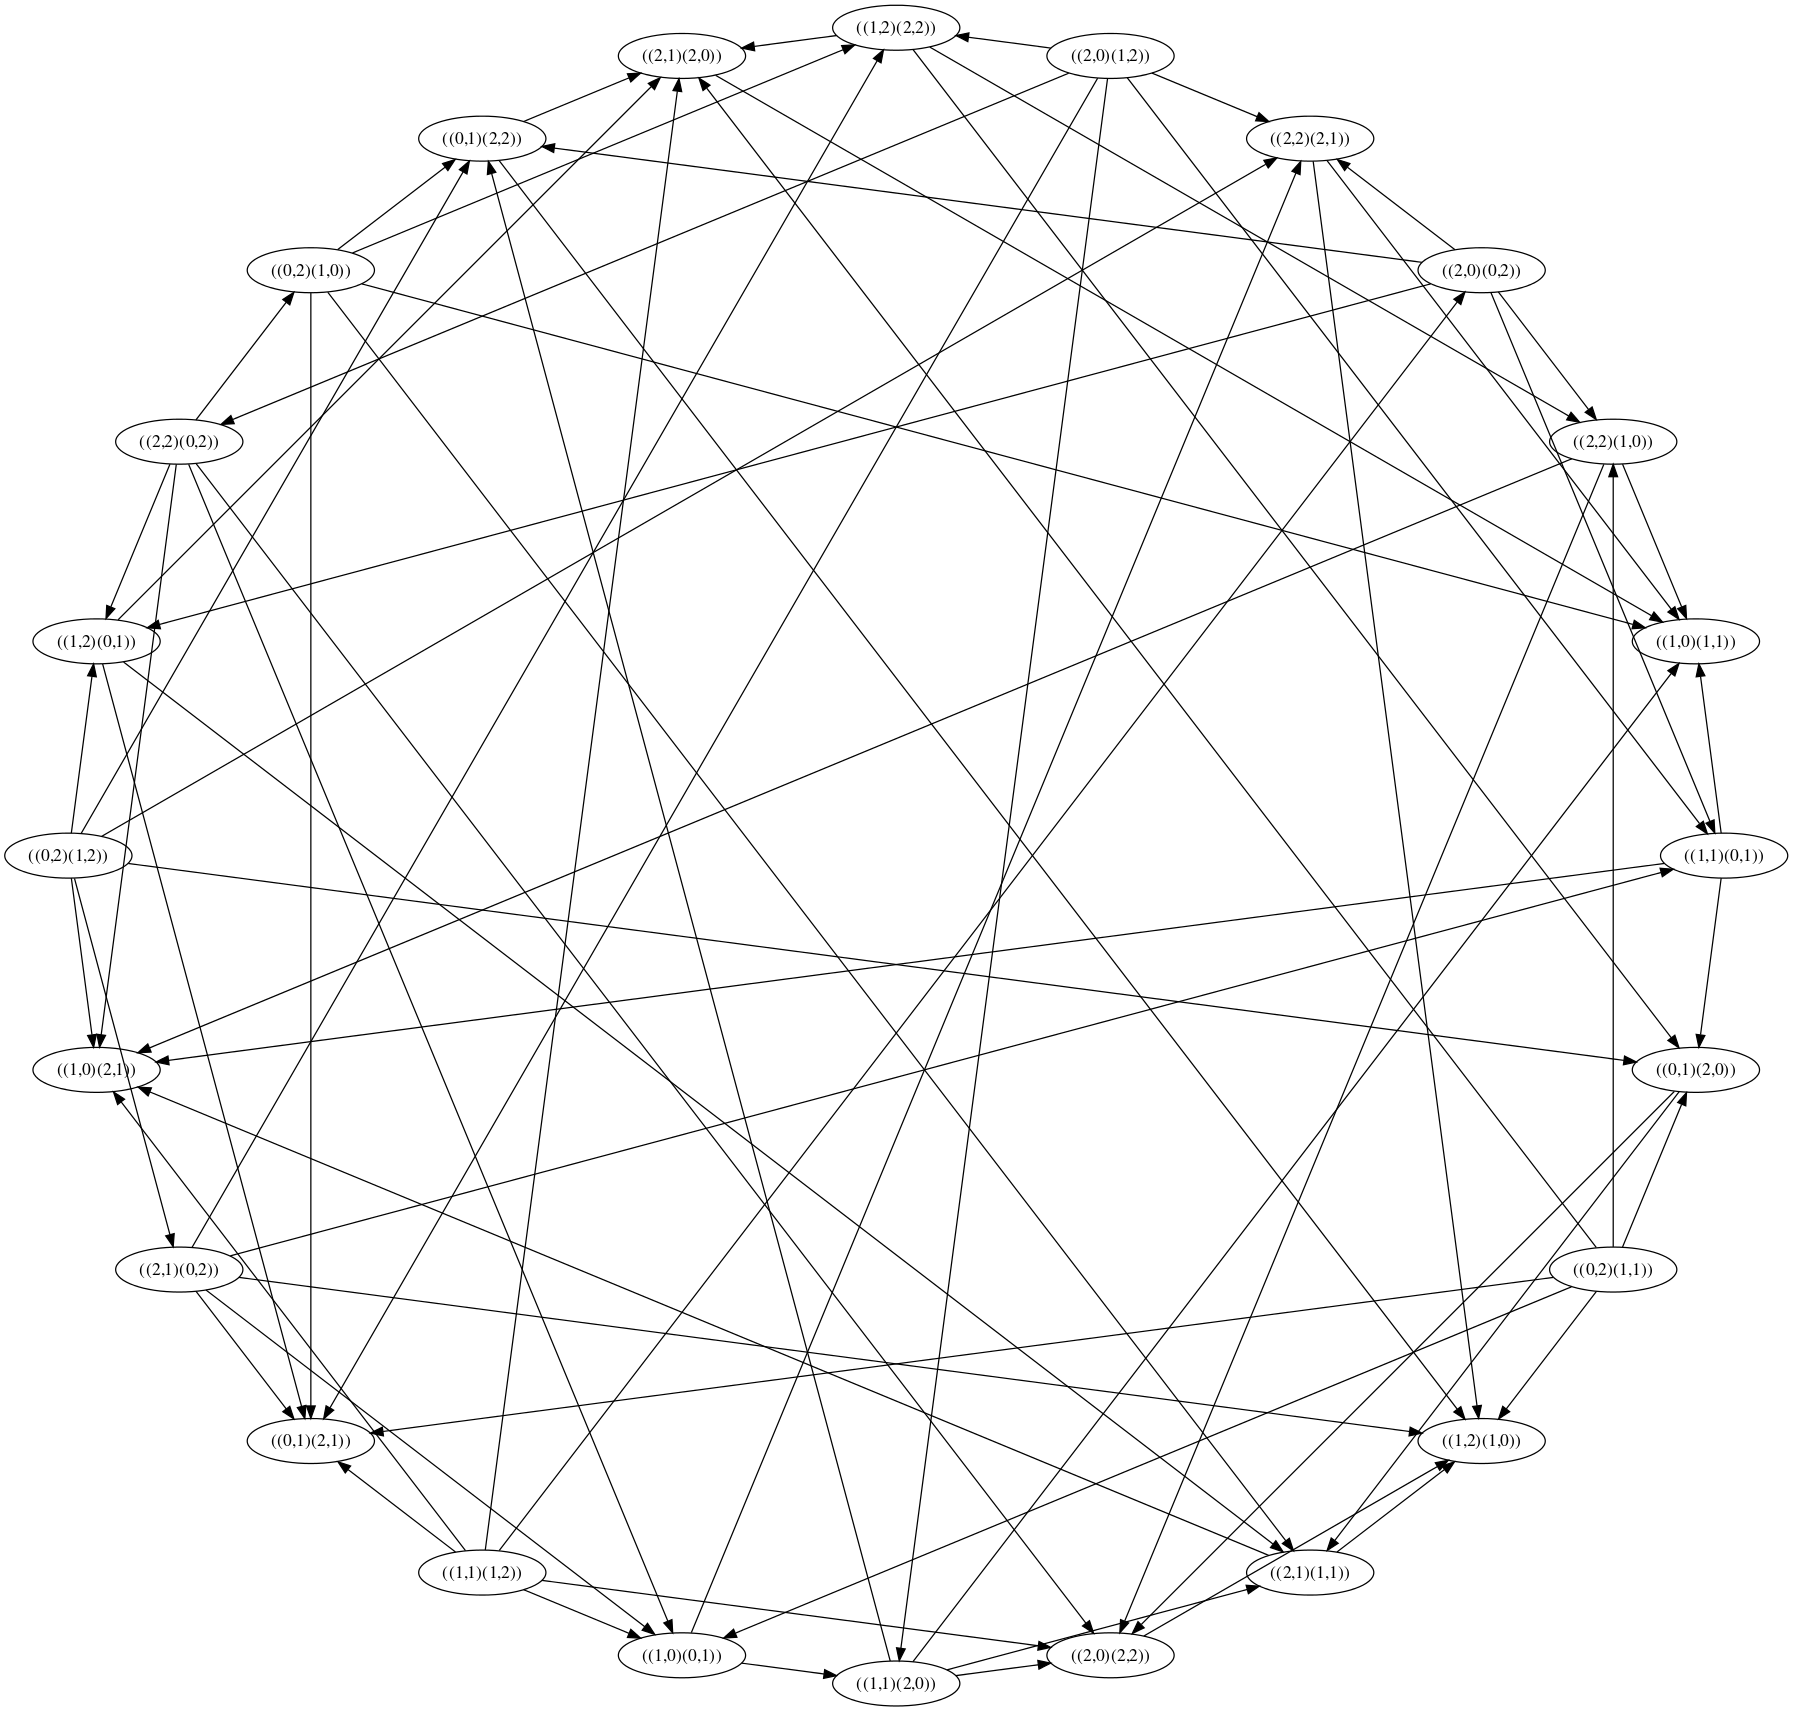
\includegraphics[scale=0.25]{example.png}
	\caption{ Output of circos ~\cite{Circos} of $C(SL(2,3), S)$ }
\end{figure}

The generating set $S$ of the group $G=SL(2,3)$ in this example has the form $\{ x_1,x_1^{-1},x_2,x_2^{-1},x_3,x_3^{-1}\}$. To verify that the Cayley graph $C(G,S)$ has diameter $2$ one would have to show that the set $S$ together with the identity and with all products $x_i^{\pm 1}y_j^{\pm 1}$ gives the entire group $G$.

\lstset{
	basicstyle=\footnotesize,
	tabsize=2
}

\subsection{Generation of cayley graphs with given diameter}

We present algorithm for generation of Cayley graph in the form of a pseudocode with short description. ~ \\
As an input procedure takes {\em generating\_set} in our case symmetric set of matrices. We copy all matrices into {\em stack} array functioning as a placeholder for all elements which weren't multiplied by elements from {\em generating\_set}. We make a mark on each of them in array {\em generating\_nodes} to make sure they won't get into {\em stack} again. We also put mark on first one with variable {\em current\_node}, name is a shortcut for currently generating node. Procedure continues into loop with terminantion set on empty {\em stack} array, in other words we are out of unique generating nodes. Inner loop is multiplying our marked node from stack by all elements in {\em generating\_set}. Every result is placed in two dimensional array called {\em cayley\_graph} on place of {\em current\_node} which is an array. Such assigning puts {\em result} at the end of array. Structure of {\em cayley\_graph} can be interpreted as graph with indeces being nodes and array on each such node as directed edges with origing in it. Result of multiplication is then tested for uniqness in {\em if} condition by checking index in {\em generating\_nodes} array. If it's unique we put it at the end of stack and make a mark in {\em generating nodes}. Exiting inner loop we continue by throwing out first element or shift in {\em stack} and making first one {\em current\_node}. Procedure ends with returning filled up {\em cayley\_graph} structure.  ~\\

\lstinputlisting[language=Perl, frame=sinlge]{cayley_graph_generation.pl}

On lines $6,13,15,17$ we denoted by $[ result ]$  the operation of putting the resulting matrix into a so-called associative array, also known as dictionary or hash array. It's worth mentioning that there exists a perfect hash function for matrices over finite fields for such purposes.

Checking diameter of Cayley graph can be done via multiplications on {\em generating\_set}. In next part we describe algorithm for such pourpose with brief description. As an input procedure takes {\em generating\_set} and {\em diameter} we want check on graph. First we put all elements of {\em generating\_set} into {\em reached\_nodes}. Next loop iterates over all $n \in \{2 \dots diameter\}$. While inner loop iterates over all variations with repetition of indeces of length $n$ from {\em generating\_set}. We assign each variation to array {\em var} and multiply {\em generating\_set} elements in same order as saved indeces in {\em var}. We put multiplicatoin result into {\em reached\_nodes}. After exiting inner loop we get all multiplication results we want of length $n$ with it's possible wheter Cayley graph has diameter {\em n}. Graph has diameter {\em n} if we got all nodes of Cayley graph. Our function checks all diameters up to {\em diameter}. If algorithm fails to return any diameter graph has bigger one. Algorithm doesn't deal with case of diameter $1$ which can be done by checking degrees on each vertex on Cayley graph. case for checking graphs with diameter $2$. Only after confirmation that our algorithm will produce all nodes we have to generate graph and check degree of vertices. ~\\

\lstinputlisting[language=Perl, frame=sinlge]{check_diameter.pl}

Implementation of algorithms is done in the {\em Perl} programming language. Perl is high-level, general-purpose, interpreted programming language with great documentation and online community maintaining easy to use libraries. While Perl being high-level programming language, multiplication of matrices in our program were actually implemented in C programming language. For this purpose we have used the library called PDL or perl data language available at {\em CPAN}~\cite{CPAN}.

\subsection{Computer search of graphs with diameter $2$}

We tested the above code on a group, $G=SL(2,5)$, of order $120$. By the Moore bound for diameter $2$ the first feasible size of a symmetric unit-free generating set $S$ is $|S|=12$.
 
To have an idea how big the task of checking all such subsets be, let us make a calculation. The group $G$ has exactly one involution and so $118$ non-involutory elements coming in pairs (an element with its inverse). So, one has a set $118/2=59$ elements (containing no inverse pair) to choose from. Assuming that our set $S$ does not contain an involution, we would have to test all choices of $12/2=6$ elements from a set of $59$ elements, which means testing ${59 \choose 6} = 45057474 $ cases, that is, more than 45 million of possibilities (and this is just a lower bound). This shows that even this modestly looking case is computationally demanding (when taking into account that after a set has been chosen one still has to test for diameter)
 
Since the numbers would increase dramatically for larger degrees we decided to restrict ourselves to a random search for suitable generating set $S$ that would give     a Cayley graph $C(G,S)$ of diameter $2$. The following table summarizes our random search results for generating sets $S$ of size $d$ for the group $G=SL(2,5)$ such     that the Cayley graph $C(G,S)$ has diameter $2$: ~ \\
 
\begin{tabular}[htbp]{l*{10}{c}r}
     $d$ & $12$ & $13$ & $14$ & $15$ & $16$ & $17$ & $18$ & $19$ & $20$ & $21$ \\
\hline
     Found graphs & $0$ & $0$  & $0$ & $1$ & $107$ & $345$ & $2451$  & $4120$ & $11669$ & $14926$ \\
\end{tabular} \\ \\

 We also run our randomized algorithm to find Cayley graphs of relatively small degree and diameter $2$ for the next group in this family, $SL(2,7)$, of order $336$.The same approach was used on Cayley graphs for the group $SL(2,7)$ with order of $336$ with Moore bound giving the minimum value of $d=19$. We have searched $150000$ graphs on each degree from $20$ to $30$ with only $10$ graphs found on $d=30$. Again, $20$ is the first realistic degree to try, but now the number of possibilities to search through is astronomical. Indeed, by a similar calculation as illustrated above, one would obtain ${167\choose 10} = 3532580013585348$ possibilities! Thus, for a randomized search such a small number of resulting graphs is not a surprise.
 
As already mentioned, we could not find results (or a code) related to the degree/diameter problem for special linear groups. On the other hand, such groups play an     important role in the study of symmetric discrete structures, which makes them prime candidates to be tested in the context of the degree/diameter problem as well.

In later stages program was modified to find any graph with diameter 2 even in groups with bigger order by making restrictions on computations. The program needs to be set up with starting size of a generating set, time limit spent per degree, maximum of generated graphs per degree and number of parallel processes. In order to find some graph with diameter $2$ the program tries to find any graph of a given  degree In the case when the time limit is reached, the program continues to work with a generating set of a bigger size. After first successfuly found graph the search continues by making generating set smaller with bigger time limit spent on degree.

Tu pojdu vysledky z hladania lepsich grafov zo Zp 11, 13, 19

For comparsion we present latest known results for Cayley graphs with $k=2$
\begin{center}
	\scalebox{0.6}{
		\begin{tabular}{| l | l | l | l | l | l |}
			\hline
			$d$ & Order & \% Moore Bound & 			$d$ & Order & \% Moore Bound \\ \hline
			$4$ & $13$ & $76.47\%$ & 				$31$ & $648$ & $67.35\%$ \\ \hline
			$5$ & $18$ & $69.23\%$ &       			$32$ & $648$ & $63.21\%$ \\ \hline
			$6$ & $32$ & $86.48\%$ &       			$33$ & $648$ & $59.44\%$ \\ \hline
			$7$ & $36$ & $72\%$ &       			$34$ & $648$ & $56\%$ \\ \hline
			$8$ & $48$ & $73.48\%$ &       			$35$ & $648$ & $52.85\%$ \\ \hline
			$9$ & $60$ & $73.17\%$ &       			$36$ & $648$ & $49.96\%$ \\ \hline
			$10$ & $72$ & $71.28\%$ &       			$37$ & $800$ & $58.39\%$ \\ \hline
			$11$ & $84$ & $68.85\%$ &       			$38$ & $800$ & $55.36\%$ \\ \hline
			$12$ & $96$ & $66.20\%$ &       			$39$ & $800$ & $52.56\%$ \\ \hline
			$13$ & $112$ & $65.88\%$ &       			$40$ & $968$ & $60.46\%$ \\ \hline
			$14$ & $128$ & $64.97\%$ &       			$41$ & $968$ & $57.55\%$ \\ \hline
			$15$ & $144$ & $63.71\%$ &       			$42$ & $968$ & $54.84\%$ \\ \hline
			$16$ & $200$ & $77.82\%$ &       			$43$ & $968$ & $52.32\%$ \\ \hline
			$17$ & $200$ & $68.96\%$ &       			$44$ & $968$ & $49.97\%$ \\ \hline
			$18$ & $200$ & $61.53\%$ &       			$45$ & $1058$ & $52.22\%$ \\ \hline
			$19$ & $200$ & $55.24\%$ &       			$46$ & $1152$ & $54.41\%$ \\ \hline
			$20$ & $210$ & $55.36\%$ &       			$47$ & $1152$ & $52.12\%$ \\ \hline
			$21$ & $288$ & $65.15\%$ &       			$48$ & $1152$ & $49.97\%$ \\ \hline
			$22$ & $288$ & $59.38\%$ &       			$49$ & $1352$ & $56.28\%$ \\ \hline
			$23$ & $392$ & $73.96\%$ &       			$50$ & $1352$ & $54.05\%$ \\ \hline
			$24$ & $392$ & $67.93\%$ &       			$51$ & $1352$ & $51.96\%$ \\ \hline
			$25$ & $392$ & $62.61\%$ &       			$52$ & $1352$ & $49.98\%$ \\ \hline
			$26$ & $392$ & $57.90\%$ &       			$53$ & $1458$ & $51.88\%$ \\ \hline
			$27$ & $392$ & $53.69\%$ &       			$54$ & $1568$ & $53.75\%$ \\ \hline
			$28$ & $512$ & $65.52\%$ &       			$55$ & $1568$ & $51.81\%$ \\ \hline
			$29$ & $512$ & $60.80\%$ &       			$56$ & $1568$ & $49.98\%$ \\ \hline
			$30$ & $512$ & $56.82\%$ &       			$57$ & $1682$ & $51.75\%$ \\ \hline
		\end{tabular}
	}
\end{center}

\section{The degree/girth problem}
Finding regular graphs with smallest possible order denoted $n_{d,g}$ with given degree $d$ and girth $g\geq3$ is known as {\em degree/girth problem}. Motivation for finding such graphs could arise from constructing graphs with no cycles of length less than $g$ and its similarity to {\em degree/diameter problem}. The problem was studied first by Biggs ~\cite{Biggs}.
\subsection{Moore bound}
For odd $g$ we have the Moore bound denoted by $M_{d,g}$
\begin{equation*}
	n_{d,g} \geq M(d,g) = 1 + d + d(d - 1) + d(d - 1)^{2} + \dots + d(d - 1)^{\frac{g-3}{2}}
\end{equation*}	
and for even $g$
\begin{equation*}
	n_{d,g} \geq M(d,g) = 2(1 + (d - 1) + (d - 1)^{2} + \dots + (d - 1)^{\frac{g-2}{2}})
\end{equation*}	

For odd $g$ the Moore bound is obtained in the same way as the Moore bound for the degree/diameter problem for the diameter $k=(g-1)/2$. For even $g$ we start with an edge and from its incident vertices we continue growing two spanning trees until we reach depth $(g-2)/2$.
\subsection{Moore graphs}
Graphs of degree $d$ and girth $g$ with order equal to $M(d,g)$ are called Moore graphs or cages. We list all cases with $n_{d,g} = M_{d,g}$ below:

\begin{itemize}
	\item{\makebox[2cm]{For $d=2$,\hfill}$g \geq 2$ - circles}
	\item{\makebox[2cm]{For $g=3$,\hfill}$d \geq 2$ - complete graphs}
	\item{\makebox[2cm]{For $g=4$,\hfill}$d \geq 2$ - complete bipartite graphs}
	\item{\makebox[2cm]{For $g=5$,\hfill}$d=2$ - circle of length $5$}
	\item[]{\makebox[2cm]{\hfill}$d=3$ - Peterssen graph}
	\item[]{\makebox[2cm]{\hfill}$d=7$ - Hoffman-Singleton graph}
	\item[]{\makebox[2cm]{\hfill}$d=57$ - this value has not been excluded but no such graph has been found yet }
	\item{\makebox[3cm]{For $g \in {6,8,12}$,\hfill}if $d-1$ is a prime power}
\end{itemize}

\begin{figure}[!ht]
	\centering
	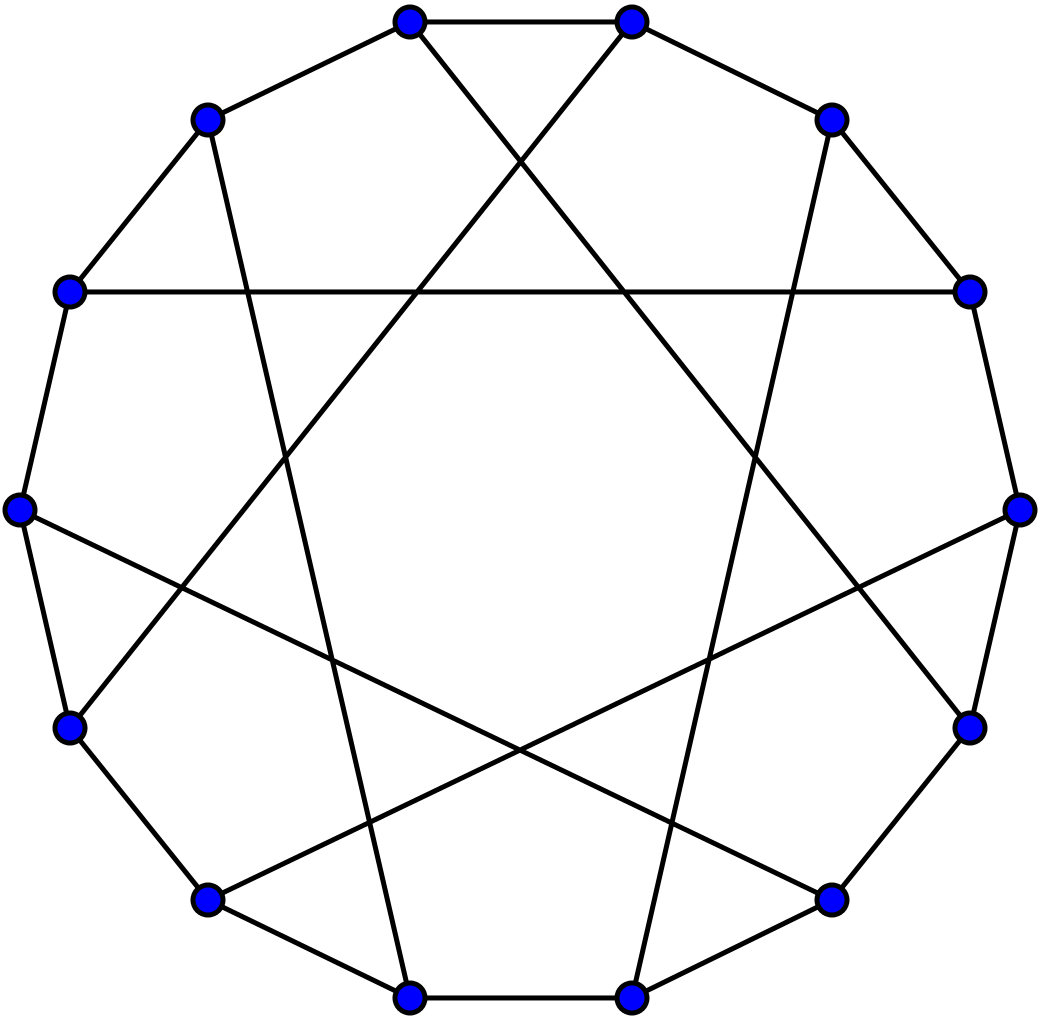
\includegraphics[scale=0.15]{Heawood_graph.png}
	\caption{The Heawood graph is a Moore graph with $d=3$ and $g=6$ }
\end{figure}

\subsection{Example of a Cayley graph ***specify parameters***}
Here we present an example of a Cayley graph on the group $SL(2,3)$ of order $|SL(2,3)|=24$

\subsection{Generation of Cayley graphs with given girth}

As in the case of diameter, for determining the girth of a Cayley graph it is sufficient to consider only multiplication by elements of the generating set.
To conclude that a graph has girth $g$ it is sufficient to have a cycle of length $g$ but no cycles of any smaller length. 
Here we present our algorithm used for computation of the girth of a Cayley graph. We divided algorithm into two procedures with finding cycles of graph and one making decision about size of girth. 
We start by {\em check\_girth} procedure taking generating set and looking size of girth on graph. 
At the beginning call {\em find\_cycle} procedure with {\em girth} we are trying to find. In case we found any cycle with such length we have to check all cycles with $length \in \{3 \dots girth - 1\}$. Any success in in condition on line $15$ results with returning girth of graph smaller than {\em girth}. In case we couldn't find any of them graph has given girth.

Procedure {\em find\_cycle} taking same arguments is iterating over all variations with repetition with order of {\em girth} and assigning indeces into {\em var} array. Multiplication result is made by multiplying elements of {\em generating set} in same order as in {\em var}. Imidiatelly after we got our result we check wheter it's neutral element. If condition is true we have found cycle with length of {\em girth}. False for all cases gives as negative result for such cycle.

\lstinputlisting[language=Perl, frame=sinlge]{check_girth.pl}

\newpage

\section{Conclusion}

In our work we discussed problems of construction of graphs with restriction on {\em degree/diameter} and {\em degree/girth}. We discussed theoretical bounds on both problems called after Moore and special cases of graphs reaching the Moore bound. We introduced Cayley graphs as a special case of graphs with a `high level of symmetry'. Cayley graphs of a given degree and diameter (or girth) have been considered before, but to the best of our knowledge not on special two-dimensional linear groups. This was the reason why we tried to extend the search to such groups of comparatively small order, and to diameter 2 and small girth. We described implementation and our approach in search for such graphs with our results.

\begin{thebibliography}{xx}

\bibitem{Bas-Mil} E. T. Baskoro and M. Miller, On the construction of networks with minimum diameter,
Australian Computer Science Communications C 15 (1993) 739?743.

\bibitem{Bev-Ers} D. Bevan, G. Erskine and R. Lewis, Large circulant graphs of fized diameter and arbitrary degree, Ars Math. ontemp. 13 (2017), 275--29.

\bibitem{Erd-Faj} P. Erd{\H o}s, S. Fajtlowicz and A.J. Hoffman,
Maximum degree in graphs of diameter 2, Networks 10
(1980), 87--90.

\bibitem{Exo-Jaj} G. Exoo and R. Jajcay, Dynamic cage survey, Electr. J. Combin. 15 (2008), Dynamic Survey DS16.

\bibitem{Gro-Tuc} J. L. Gross and T. W. Tucker, Topological Graph Theory. Wiley, 1987 and Dover, 2001.

\bibitem{Hof-Sin} A. J. Hoffman and R. R. Singleton, On Moore graphs with diameter $2$ and $3$, IBM J. Res. Develop. 4 (1960), 497--504.

\bibitem{Mil-Sir} M. Miller and J. \v{S}ir\'a\v{n},  Moore graphs and beyond: A survey, 2nd Ed., Electr. J. Combin. 2013, Dynamic Survey DS15.

\bibitem{Sia-Sir} J. \v{S}iagiov\'a and J. \v{S}ir\'a\v{n}, Approaching the Moore bound for diameter two by Cayley graphs, J. Combin. Theory Ser. B 102 (2012) 470--473.

\bibitem{Biggs} N.I. Biggs, Girth, valency and excess, Linear Algebra Appl. 31 (1980) 55-59

\bibitem{Circos} Circo, http://circos.ca

\bibitem{CPAN} PDL, https://metacpan.org/pod/PDL

\end{thebibliography}

\end{document}
